\section{\Sys Design}
\label{sec:methodology}

\Sys, illustrated in Figure \ref{arch}, is composed of five key modules: a provenance graph constructor, a Federated Averaging server, a utility server, and client machines. At a high-level, \Sys generates provenance graphs from system logs, uses semantic attributes to create feature vectors for nodes, and applies \gnnshort for context-aware encoding. These embeddings are stored in a database and later used by a lightweight classifier during threat detection.

\begin{figure}[t!]
    \centering
    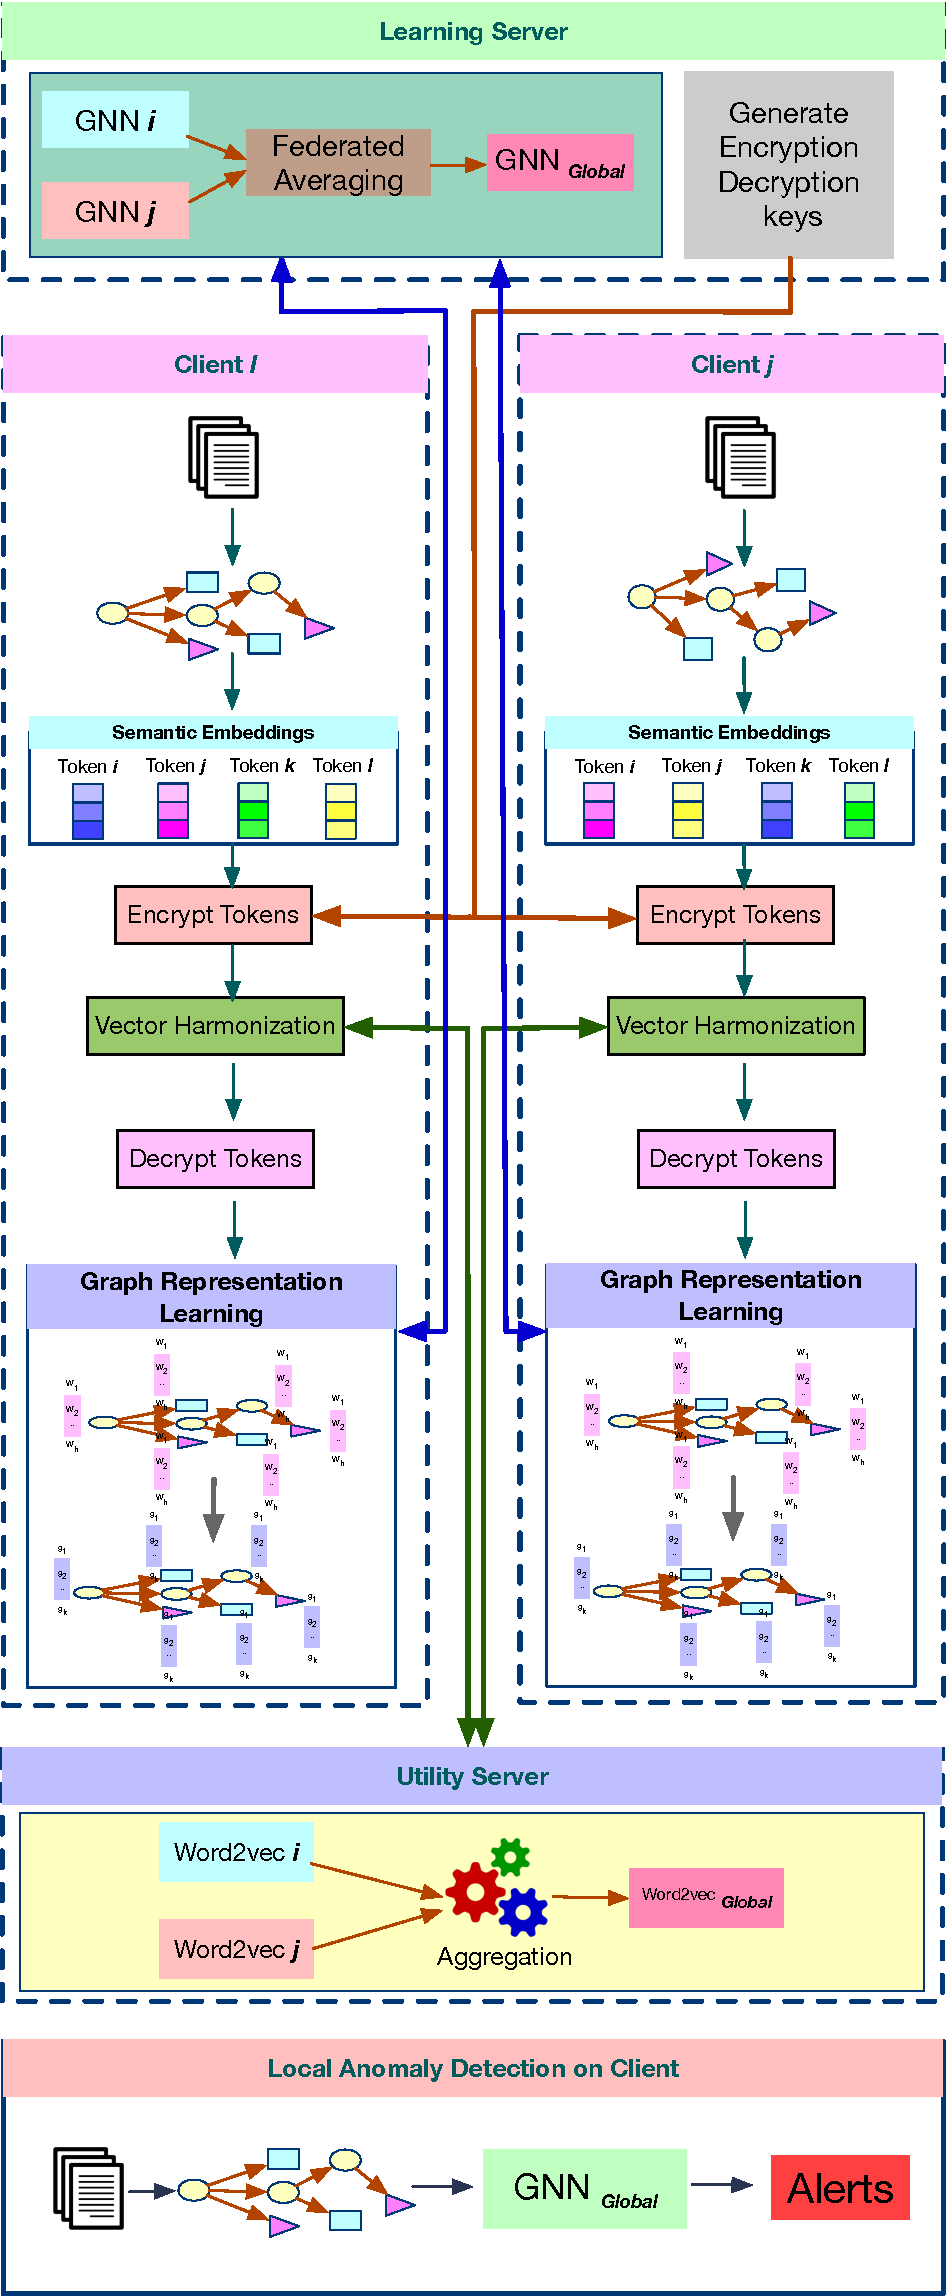
\includegraphics[width=0.45\textwidth]{fig/arch.pdf}
    \caption{High Level Architecture of \Sys}
    \vspace{-3ex}
    \label{arch}
  \end{figure}
